\chapter{People detection}
Under this section, the solution adopted for the vision-based human detection part of the project, the arguments that led to this approach, the assumptions made, the tests performed and the obtained results are presented. 

\section{Problem definition}
Once the purpose of the vision system has been well defined, the operating conditions and the environment must be carefully studied in order to find the most suitable solution.
An embedded vision system portable by a drone, robust and fast enough and with low energy consumption is required for the task. 
The search of people in the sea entails specific problems that must be treated such as:

\begin{enumerate}[itemsep=1mm,topsep=1mm,leftmargin=.35in]
    \item False positives due to any kind of ocean animals or rocks
    \item Changes in illumination conditions due to outdoors work
    \item Forecast behavior: wind, rain
    \item Moving background and platform
    \item Highly reflective background
\end{enumerate}%

Therefore, the election of the hardware and the vision algorithm has to be taken consequently with these points.

\section{Equipment}
According to the ideas above and the available resources, a logically consistent choice seems to go through the image processing options. 
This is due to the fact that any other kind of visual system (thermal camera, structured light, time of flight measurements, etc) do not fulfill the requirements or turns out to be too expensive.
Hence, a GoPro HERO 3 camera has been chosen as a robust, light and powerful enough solution \cite{ref:HERO3}.
In order to deal with the instability and disruptions caused by the platform, the camera has been mounted on a Tarot T-2D Brushless Gimbal Kit, whose technical details can be found in \cite{Ref:Gimbal}, which used as a stabilizer.

\subsection{GoPro HERO 3}
The technical parameters of the chosen camera model have influenced the way the vision algorithm has been approached.
The characteristic small focal length of this camera model, together with the flight altitude of the drone, leads to a wide field of view, and therefore a big scanned area of ocean per frame. 
The high resolution of the frames allows a precise image processing with a low loss of information in the acquisition even from high altitude.
Its elevated frame rate for video is, however, constrained by the processing time of the vision algorithm, which has been developed striving for low memory and time consumption since it processes the images online and its aimed to do it onboard.

\subsection{GoPro gimbal}
The installed gimbal Tarot T-2D Brushless Gimbal Kit offers roll and tilt stabilization and has been configured to point the camera downwards due to its wide FOV. 
By doing this it is ensured that once the drone is offshore the images will only contain a background of the ocean, facilitating the image processing and speeding up the preprocessing of the pictures.
Furthermore, as said before, the gimbal provides high stability for precise image acquisition and filters out disruptions on the flight, which allows an easier and more reliable human detection system.


\section{Vision task}
Given the hardware platform, the image processing algorithm must deal with the remaining problems in order to reach the goal of the system. 
The initial proposals for people detection, based on movement analysis and human morphological features extraction where discarded after being subjected to more detailed studies. 
The moving platform and the waves made unfeasible a reliable solution based on movement tracking assuming that the people to be found were moving.
Furthermore, the possibility of the targets being drowning, partially or almost completely covered by water prevented any kind of solution from succeeding employing morphological analysis. 
In the view of the arguments above, the final solution was decided to perform human skin detection based on color under the assumption that at least a part of the targets would be floating. 


\subsection{Human skin identification}
In order to perform a robust detection, the RGB-H-CbCr human skin color model presented in \cite{Ref:SkinColorModel} and \cite{Ref:SkinDetection} has been implemented in the algorithm and applied for image thresholding as introduced in \cite{Ref:SkinDetection}. This filter has been added to overcome the issue issue of occlusion, which will occur as the drone is patrols crash site and wreckage might occlur with victims, and thereby making it harder to detect them. The filter has been trained by looking at 140 different skin color patches, from which the color model has been made. The filter robust against  various levels of brightness and illumination, which is an favouable feaure for this application as the wheather condition cannot be predicted,and also affect how the skin color of a person is perceived. 
%\begin{equation}
%		\begin{cases}
%		    (R > 95) AND (G > 40) AND (B > 20),& \text{AND}\\
%		    (max(R, G, B) - min(R, G, B) > 15), & \text{AND}\\
%		    (abs(R - G) > 15) AND (R > G) AND (R > B)
%		\end{cases}
%		\label{eq:rule1}
%\end{equation}
%\begin{equation}
%		\begin{cases}
%		    (R > 220) AND (G > 210) AND (B > 170),& \text{AND}\\
%			(|R - G| <= 15) AND (R > B) AND (G > B)
%		\end{cases}
%		\label{eq:rule2}
%\end{equation}

%\begin{equation}
%		\begin{cases}
%			Cr ≤ 1.5862 × Cb + 20
%			Cr ≥ 0.3448 × Cb + 76.2069
%			Cr ≥ -4.5652 × Cb + 234.5652
%			Cr ≤ -1.15 × Cb + 301.75
%			Cr ≤ -2.2857 × Cb + 432.85
%			\end{cases}
%		\label{eq:rule3}
%\end{equation}

%\begin{equation}
%		\begin{cases}
%			H < 25
%			H > 230
%		\end{cases}
%	\label{eq:rule3}
%\end{equation}
The filter is applied after input has been binary segmented and  ROI's of the white blobs has been made. Each ROI will will run through the filter, and if the filter deems the ROI to contain a human will it be noted otherwise ignored.  By only working on ROI images rather than the full image, is the computational time needed for apply the filter shrinken to a minimum. The filter is applied on every pixel of the image, the response of the pixel is saved in a map. If the filter reponse deems the pixel to be something from a human it will output a white pixel if not a it will output a black pixel.  If the pecentage of white pixels is above a threshold value, will it deemed as a human. \ref{fig:ROIs} and \ref{fig:responsemap}. 

\begin{figure}[H]
\centering
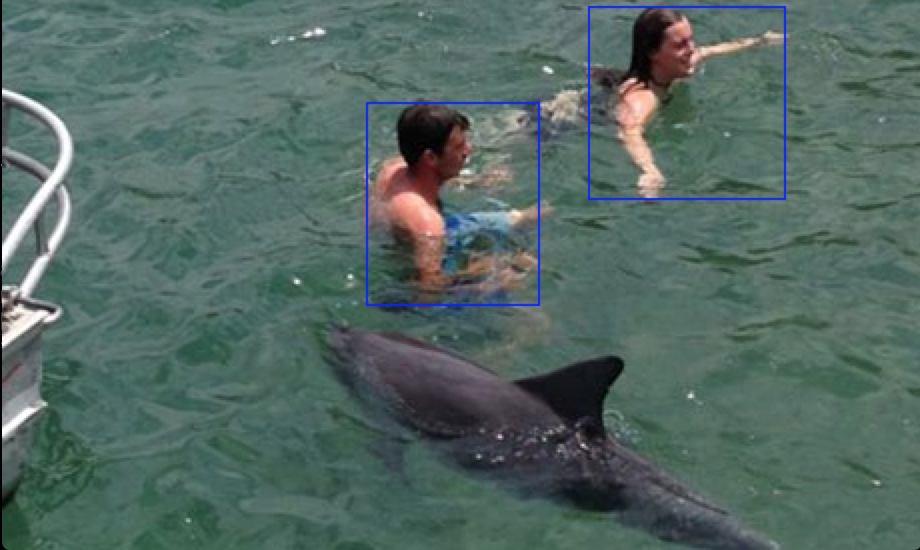
\includegraphics[width=\textwidth]{Images/humanDolphin.png}
\label{fig:humanAndDolphin}
\caption{Skin detector capable of distinct between animals and human}
\end{figure}
\begin{figure}[H]
        \centering
        \begin{subfigure}[b]{0.3\textwidth}
        	\centering
				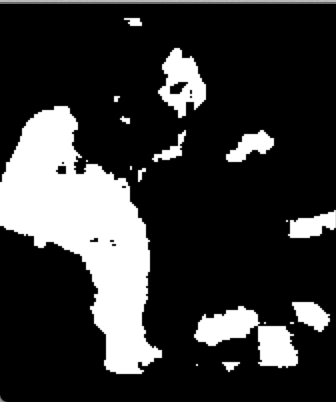
\includegraphics[scale=0.5]{Images/roi_response1.png}
        \end{subfigure}%
        \begin{subfigure}[b]{0.3\textwidth}
        	\centering
				
\includegraphics[scale=0.5]{Images/roi_response2.png}
        \end{subfigure}
        \label{fig:responsemap}
        \caption{Response map of the  detected ROI}
\end{figure}
Ordinary detector such as HaarCascades etc. are trained to detect peope within certain pose, as this a factor which cannot be kept consistent in this application the choise  of applying this detector seemed reasonable. CPU wise is the process of detection people from the footage kept at minimum meaning, meaning any computer would without problem run this program at with ease make use of its capabilities, which other trained filters may comsume alot of CPU which may inflict dificulties for the user to make use of this application.  This application could because of it's light CPU usage be implemented on the drone, but due to battery consumption of an computer running,  and not knowing the complexity of the issue, was this initial not thought as the final product. 


\subsection{Preprocessing}
The pixel-wise searching method is a very accurate but heavy process that entails a high time consumption.
In order to speed the overall performance up, some regions of interest in the image with higher possibilities of containing people must be found as a previous step. To do so, an analysis and comparison of example images of the ocean, with and without people and under different illumination conditions was carried out.  

A first approach to this consisted in filtering in the frequency domain in order to remove constant low frequencies, which would be, in this case, related to the background. Thus, only the high frequency objects would be left, containing all the isolated candidates for the detector.
Notwithstanding, it turned out that a simpler and faster threshold in the hue color space could be set up to distinguish between floating objects and the background water in all the images. 
These floating objects always involved a disruption or change in the average hue level of the whole picture, that otherwise remained constant (except for strong glare cases, which will be treated below).
However, a threshold value in hue could not be fixed, due to its dependency with the general illumination level. 
Thus, the solution adopted was to set up a dynamic threshold applying Otsu's method, as described in \cite{Ref:Otsu}.
Proceeding this way, a few small regions containing all the candidates could be input to the skin scan process, getting rid of the majority of the image with no relevant information. 
This part of the process contains the strongest assumption made for the algorithm. 
For the binarization of the image an uniform background is assumed, meaning that this step will tend to fail for images with strongly non-homogeneous surroundings. 
It can handle ocean and sky or distant coast lines tough. 

Furthermore, an estimation was made here concerning the size of the input ROIs. 
According to the hight of the drone on the flight and the focal length of the camera, an approximate calculation of the size of the pixel are of people in the image can be made. 
With it all the objects out of this boundaries can be filtered out, easing the posterior process.

As the last point on the preprocessing part, a simple and easy to implement method for dealing with the glare of the sun light on the water is suggested here, although not implemented in the project, since we came out with this problem at the very end.
The thresholding in hue was proved to fail in the cases of light reflection on small spots for certain intensities, since this glare caused also a strong enough change in the hue image histogram. To eliminate these false positives, the easiest solution would be to include a polarizer filter in the setup, which could also facilitate the color detection. 

\subsection{Postprocessing}
The outputs of the whole process are the images considered to contain people on the water in the patrolled area. 
These pictures are stored and sent to the ground control to be analyzed by the staff in charge, introducing a human in the control loop.
If the pictures are confirmed to contain people, this means that they are swimming in a forbidden zone or drowning, and the specific intervention activities are triggered, while the drone keeps its patrol. 

\section{Performance tests}
The design and implementation of the vision algorithm, developed in C++ and OpenCV, has been an iterative process consisting in several steps of coding and testing of the different parts of the program. 
For testing purposes, a database with several relevant images and videos that fulfilled the specifications for the application has been created. %(some how citation to all images on git and dropbox as it being the database of image)

A database with relevant images and videos was created with testing purposes.\\

Example of successful test in the PC for the analysis of images carried out

\begin{figure}
        \centering
        \begin{subfigure}[h]{0.3\textwidth}
                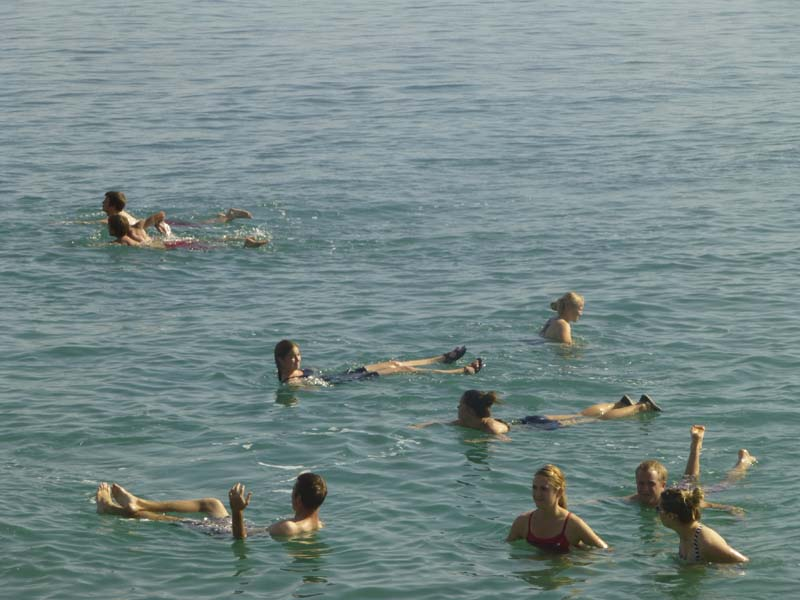
\includegraphics[width=\textwidth]{Images/ocean7}
                \caption{Image 1: original image}
                \label{fig:original}
        \end{subfigure}%
        \quad
        \begin{subfigure}[h]{0.3\textwidth}
                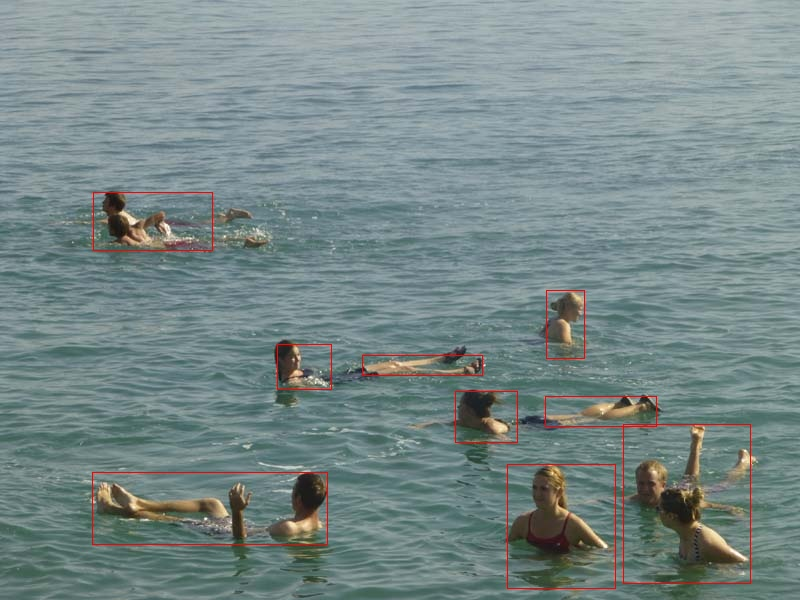
\includegraphics[width=\textwidth]{Images/final}
                \caption{Image 1: processed image}
                \label{fig:final}
        \end{subfigure}
        \caption{Original and processed images}
\end{figure}

\begin{figure}
        \centering
        \begin{subfigure}[b]{0.3\textwidth}
                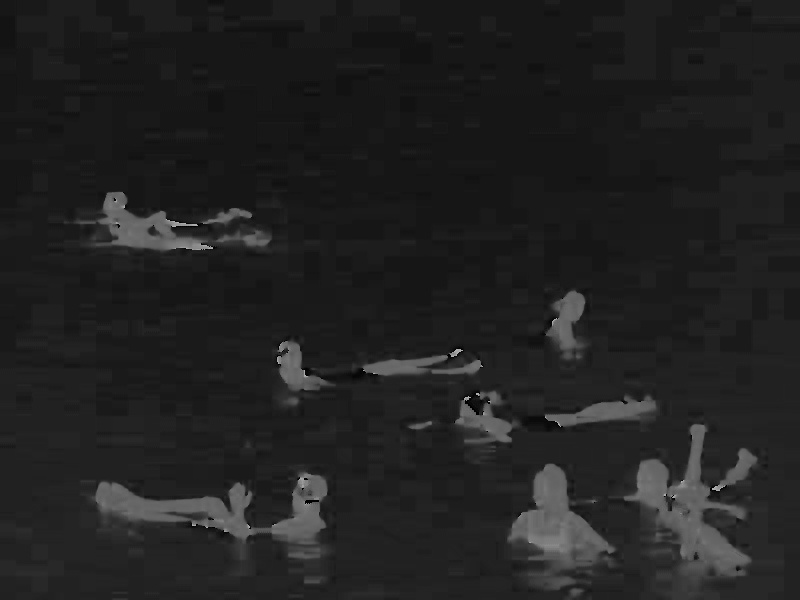
\includegraphics[width=\textwidth]{Images/hue}
                \caption{Image 1: hue}
                \label{fig:original}
        \end{subfigure}%
        \quad
        \begin{subfigure}[b]{0.3\textwidth}
                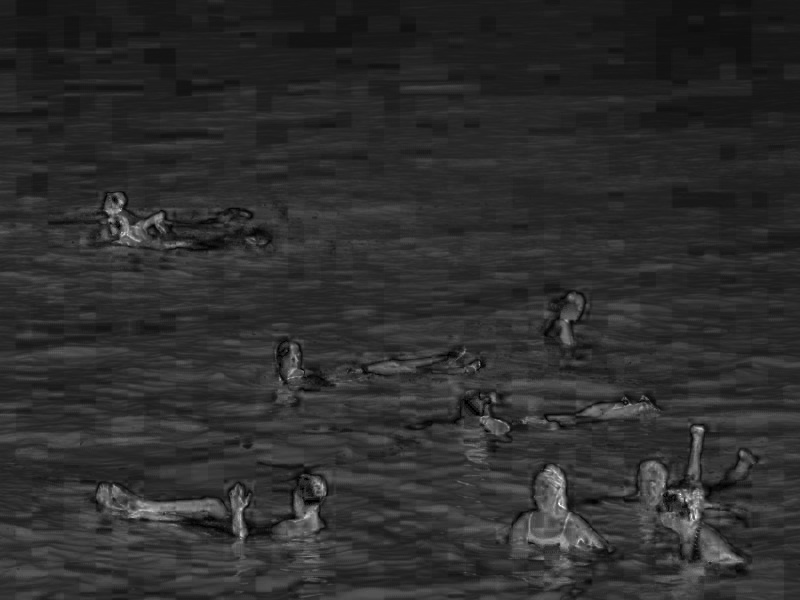
\includegraphics[width=\textwidth]{Images/sat}
                \caption{Image 1: saturation}
                \label{fig:final}
        \end{subfigure}
        \quad
        \begin{subfigure}[b]{0.3\textwidth}
                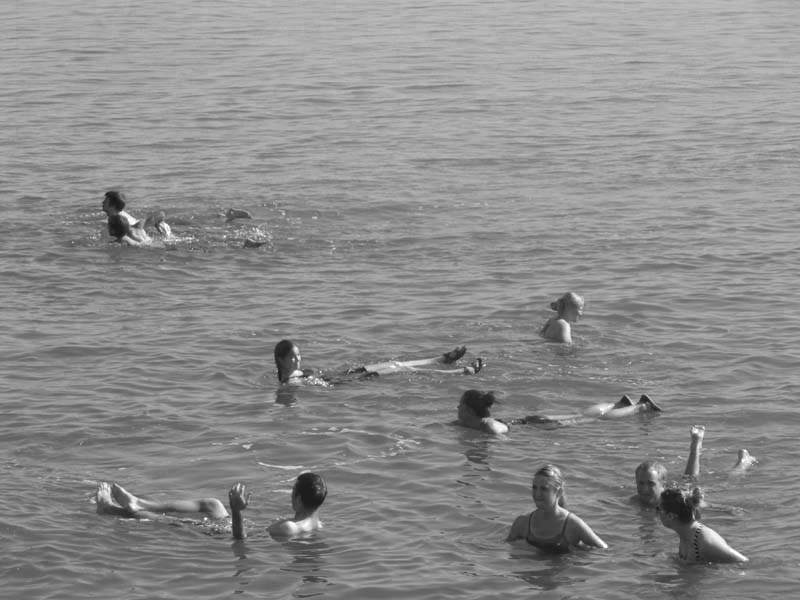
\includegraphics[width=\textwidth]{Images/val}
                \caption{Image 1: value}
                \label{fig:final}
        \end{subfigure}
        \caption{HSV color space decomposition}
\end{figure}

\begin{figure}
        \centering
        \begin{subfigure}[b]{0.3\textwidth}
                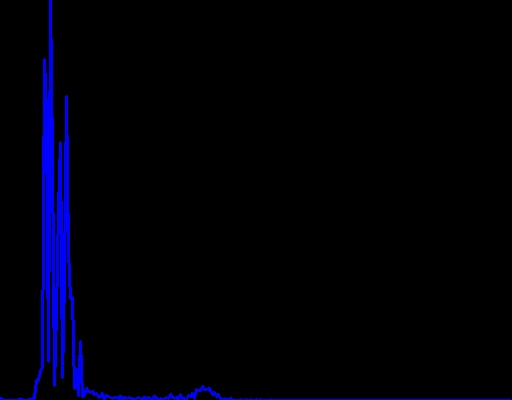
\includegraphics[width=\textwidth]{Images/hueHist}
                \caption{Image 1: hue histogram}
                \label{fig:hueHist}
        \end{subfigure}%
        \quad
        \begin{subfigure}[b]{0.3\textwidth}
                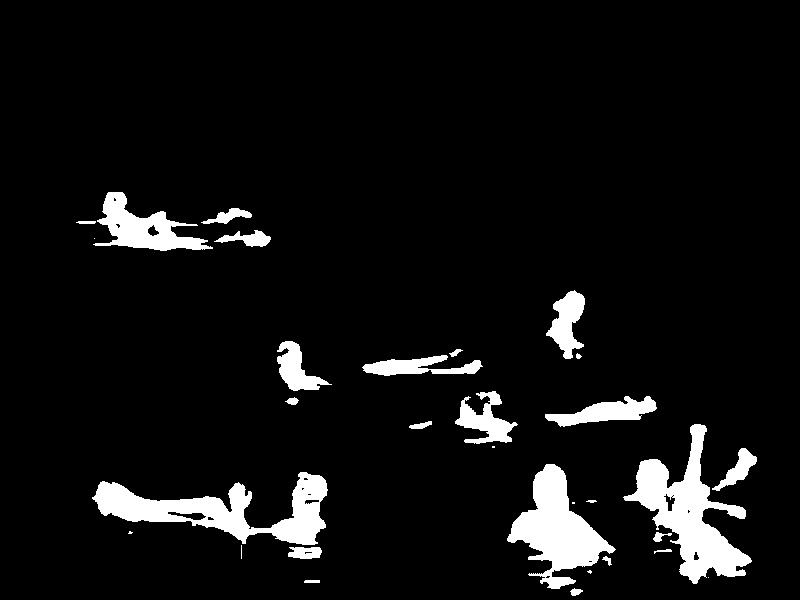
\includegraphics[width=\textwidth]{Images/bin}
                \caption{Image 1: binarized}
                \label{fig:binarized}
        \end{subfigure}
        \caption{Dynamic thresholding in hue}
\end{figure}

\begin{figure}
        \centering
        \begin{subfigure}[b]{0.3\textwidth}
                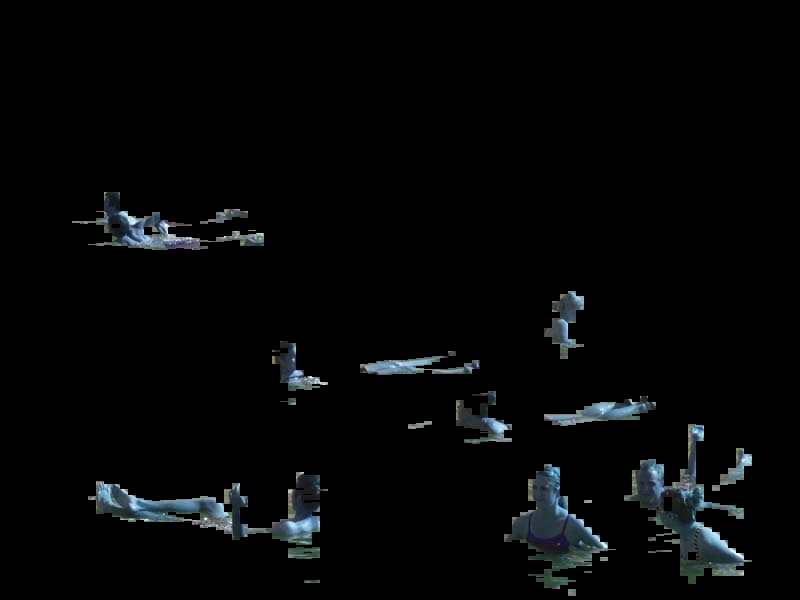
\includegraphics[width=\textwidth]{Images/proc}
                \caption{Image 1: ROIs before particles filtering}
                \label{fig:ROIs}
        \end{subfigure}%
        \quad
        \begin{subfigure}[b]{0.3\textwidth}
                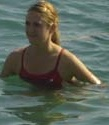
\includegraphics[width=\textwidth]{Images/ROI}
                \caption{Image 1: one of the ROIs amplified after filtering}
                \label{fig:oneROI}
        \end{subfigure}
        \caption{Dynamic thresholding in hue}
\end{figure}

\section{Results} 
%I don't maybe redundant our other section seem to have experiment data on them.. 
\section{Conclusion}
\subsection{Further work}
Implementation of the onboard communication system to send the images on the fly
\section{Discussion}
%% Some ideas for possible sections..  We should talk about it at some point.. 
\newpage